\chapter{A Closer Look at Scoring}
\label{ch:scoring}
% ##################################################################################################################

\hfill \textbf{Author:} ..., Andreas Horni, ...

\begin{center} 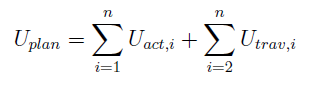
\includegraphics[width=0.3\textwidth, angle=0]{using/figures/utf.png} \end{center}

% ##################################################################################################################
MATSim scoring is a central element of MATSim. The user has the possibility to configure numerous parameters to calibrate the choice behavior. \ah{Kann man jetzt UTF im Config zusammensetzen? Rashid?} When the user is ready to extend MATSim in the next book part, he will also be able to plug in his own customized utility function.

MATSim is based on utility-maximization. Thus, estimated discrete choice models can be applied in MATSim. However, due to MATSim's iterative structure, and because it is based on complete day plans, the application of models for parts of day plans only (for example mode choice) is not straight forward as detailed in Section~\ref{sec:estimation}.

Due to the absence of a complete-day-utility function, MATSim has been started with the so-called Charypar-Nagel utility function (Section~\ref{sec:charyparnagel}) and extended for some purposes (Section~\ref{sec:utfextensions}). Readily applicable estimates for a full-day utility function is not yet available. 

% ##################################################################################################################
\section{The Current Charypar-Nagel Utility Function}
\label{sec:charyparnagel}
The first and still basic MATSim utility function was formulated by \citet[][]{CharyparNagel_Transportation_2005} from the \emph{Vickrey} model for road congestion as described in \citet[][]{Vickrey_TAER_1969} and \citet[][]{ArnottEtAl_TAER_1993}. Originally, this formulation was established for departure time choice. However, all studies performed so far, indicated that the MATSim function is also appropriate for modeling the further choice dimensions.

As in the discrete choice modeling framework (see Chapter~\ref{ch:discretechoice}), the utility $U$ is composed of a deterministic part $V$ and a random error term $\varepsilon$, i.e., $U = V + \varepsilon$. Except for destination choice the error term is not explicitly generated but stems from the random noise produced by the co-evolutionary process. Randomness is added in various ways in the process, an example is the order in which agents undergo the replanning (e.g., in which iteration choices are modified). \ah{Hier Diskussion Section~\ref{sec:discussion_scoring} noch weiter vertiefen}.

For the basic function, the utility of a plan $U_{plan}$ is computed as the sum of all activity utilities $U_{act,q}$ plus the sum of all travel (dis)utilities $U_{trav,mode, q}$:
%
\begin{equation}
\label{eq:matsimUTF}
U_{plan}=\sum^N_{q=1} U_{act,q} + \sum^{N-1}_{q=1} U_{trav, mode, q}
\end{equation}
with $N$ as the number of activities. Note that trip $q$ is the trip that follows activity $q$. The last activity does not have an associated trip, thus the sum goes only up to $N-1$

The utility of an activity $q$ is defined as follows (see also \citet[][p.377ff]{CharyparNagel_Transportation_2005}):
\begin{equation*}
U_{act,q} = U_{dur,q} + U_{wait,q} + U_{late.ar,q} + U_{early.dp, q} + U_{short.dur, q},
\end{equation*}
where:
\begin{itemize}
\item $U_{dur,q}= \beta_{dur,q} \cdot t_{typ,q} \cdot \ln(t_{dur,q}/t_{0,q})$ is the utility of performing activity $q$, where opening times of activity locations are taken into account. $t_{dur,q}$ is performed activity duration, $\beta_{dur,q}$ is marginal utility of activity duration for its typical duration $t_{typ,q}$ and $t_{0,q}$ is minimal duration, or in other words, the duration for which utility starts to be positive. 

\item $ U_{wait,q} = \beta_{wait, q} \cdot t_{wait,q}$ 

denotes the waiting time spent for example in front of a yet closet store, where $\beta_{wait,q}$ is marginal utility of waiting and $t_{wait,q}$ is the waiting time.
		
\item $U_{late.ar,q}= \left\{
  \begin{array}{l l}
    \beta_{late.ar,q} \cdot (t_{start,q} - t_{latest.ar,q}) & \quad \text{if $t_{start,q} > t_{latest.ar,q}$}\\
    0 & \quad \text{else}
  \end{array} \right.$
  
  specifies the late arrival penalty, where $t_{start,q}$ is the starting time of activity $q$ and $t_{latest.ar}$ is the latest possible starting time of that activity for example given by opening times.

\item $U_{early.dp} = \left\{
  \begin{array}{l l}
    \beta_{early.dp,q} \cdot (t_{earliest.dp, q} - t_{end,q}) & \quad \text{if $t_{end,q} > t_{earliest.dp,q}$}\\
    0 & \quad \text{else}
  \end{array} \right.$

defines the penalty for staying not long enough, where $t_{end,q}$ is the ending time of the activity and $t_{earliest.dp,q}$ is the earliest possible end time for activity $q$.

\item $ U_{short.dur, q} = \left\{
  \begin{array}{l l}
    \beta_{short.dur,q} \cdot (t_{short.dur, q} - t_{dur,q}) & \quad \text{if $t_{dur,q} < t_{short.dur,q}$}\\
    0 & \quad \text{else}
  \end{array} \right.$
  
  is the penalty for a too short activity, where $t_{short.dur}$ is the shortest possible duration for the activity.
\end{itemize}
%
Travel disutility is given as 
\begin{equation}
\label{eq:tdisutility}
U_{trav, mode, q} = C_{mode} + \beta_{trav, mode, q} \cdot t_{trav, q} + \beta_{c} \cdot c  + (\beta_{d, mode, q} + \beta_{c} \gamma_{d, mode}) \cdot d_{trav,q} + V_{transfer,q} \,
\end{equation} 
where:
\begin{compactitem} 
\item $C_{mode}$ is a mode-specific constant,
\item $\beta_{trav, mode, q}$ is the marginal utility of travel by mode (normally negative or zero),
\item $t_{trav, q}$ gives the travel time between location of activity $q$ and $q+1$,
\item $\beta_{c}$ is the marginal utility of money (normally positive),
\item $c$ are the monetary costs of the complete leg such as tolls or fares (normally negative),
\item $\beta_{d, mode}$ is the  marginal utility of distance (normally negative),
\item $\gamma_{d, mode}$ is the mode-specific distance cost rate (normally negative),
\item $d_{trav, q}$ is the distance traveled, and,
\item $V_{transfer, mode, q}$ are transfer penalties in public transport (normally negative).
\end{compactitem}
%
Note that the distance contributes to disutility in two ways. First, it is included in a direct manner via $\beta_{d, mode,q}$, which is natural for modes with physical efforts such as walking or cycling. Second, distance is also included monetarily via $\beta_c \cdot \gamma_{d, mode}$ which is natural for mode car or pt, where monetary costs increase dependent on distance.

Further note that travel receives an additional implicit penalty from the opportunity cost of time: If a travel time could be reduced by $\Delta t_{trav}$, the person would not only gain from avoiding $\beta_{trav}~\cdot~\Delta t_{trav}$, but also from making activities longer. The marginal utility of travel time savings is thus:
%
\[
mUTTS = - \frac{\partial}{\partial t_{trav}} U_{trav} + \frac{\partial}{\partial t_{dur}}U_{dur} 
\]
which is 
\[
mUTTS = - \frac{\partial}{\partial t_{trav}} U_{trav} +  \beta_{dur} \cdot \frac{t_{typ,q}}{t_{dur,q}} 
\]
and at the typical duration of an activity
\[
mUTTS = \beta_{trav} + \beta_{dur}.
\]
The marginal utility of travel time savings at the typical duration can be transformed to the more common value of travel time savings by division with $\beta_{c}$:
\[
VTTS = \frac{mUTTS}{\beta_{c}} = \frac{\beta_{trav} - \beta_{dur}}{\beta{c}}
\]
This is important for calibration of the utility function.

The extensions made over time to the original utility function are described in the next section. Clearly, only a few extensions made it into the default current utility function.

% ======================================================================================================================
\subsection{Parameters}
\label{sec:paramset}
The basic Charypar-Nagel scoring function is inspired by \citet[][]{ArnottEtAl_TAER_1993}, which provides an extension of the Vickrey model \citep[][]{Vickrey_TAER_1969}. Parameters are thus derived from this model by also consulting \citet[][]{ChaumetEtAl_2006}. A frequently applied parameter set is the following 
%
\begin{compactitem}
\item $\beta_{dur,q}= 6\ utils/h$,
\item $\beta_{trav, mode, q}= -6\ utils/h$,
\item $U_{wait,q}=0\ utils/h$,
\item $\beta_{short.dur,q} = 0 utils/h$
\item $\beta_{late.ar,q}=-18\ utils/h$,
\item $\beta_{early.dp,q}=-18\ utils/h$.
\end{compactitem}
%
Nowadays the utility function measures in the unit $utils$, where an earlier interpretation was based on monetary terms (e.g., $\EUR$).

%\citet[][p.164, p.173]{ArnottEtAl_TAER_1993} defines 
%$\alpha=5.00\ \$/h$ the shadow cost of travel time,
%$\beta=3.05\ \$/h$ the unit cost of arriving early at work, and
%$\gamma=11.88\ \$/h$ the unit cost of arriving late based on the estimations reported by \citet[][Table 2 on p.473]{Small_AER_1982}.
%Derived from this initial values \citet[][p.382]{CharyparNagel_Transportation_2005} define the MATSim utility function as follows, where they consider the opportunity costs of $20\ EUR/h$, i.e., the costs for doing nothing. \ah{wie genau kam man auf die Werte? \\ In \citet[][p.122]{ArnottEtAl_JUE_1990}, they are defined as $\alpha=6.40\ \$/h$, $\beta=3.90\ \$/h$ and $\gamma=15.21\ \$/h$.
%
%Bernhard and Axhausen: Metaanalysis. Normwerk. Verlässlichkeit ...
% Chaumet, R., P. Locher, F. Bruns, D. Imhof, M. Bernard and K.W.\ Axhausen (2007) Verfahren zur Berücksichtigung der Zuverlässigkeit in Evaluationen, final report for VSS 2002/002, Schriftenreihe, 1176, Bundesamt für Strassen, UVEK, Bern. 
%}

% ##################################################################################################################
\section{Extensions}
\label{sec:utfextensions}
The following paragraphs describe, how the basic utility function explained in \citet[][]{CharyparNagel_Transportation_2005} has been extended by monetary and distance costs and mode-specific travel parameters including constants. Please be aware, that the MATSim code base and in particular the scoring functionality has changed a lot in recent years, e.g., the scoring is now based on events rather than on plans \ah{...}. Thus, the historical development is accompanied by various conceptual and technical modifications leading to the current utility function described above. This also means, that the reported parameter settings are an indication not a direct recommendation.

% ======================================================================================================================
\paragraph{Project Westumfahrung Zürich:}
Project Westumfahrung \citep[][]{BalmerEtAl_ResRep_bdktzrh_2009} used the Zürich scenario version 1 \citep[][]{HorniEtAl_TechRep_IVT_2011_a}. Only car traffic was simulated with $\beta_{perf,q}=6.0\ utils/h$ and $\beta_{trav,q}=-6.0\  utils/h$. No further penalties were applied. Typical activity durations were provided with the config with half-hour resolution and empirically derived from the Swiss microcensus.

% ======================================================================================================================
\paragraph{Kickhöfer:}
\citet[][]{Kickhoefer_MastersThesis_2009} added monetary variables and income to the MATSim utility function and performed a mode-specific estimation based on the survey by \citet[][]{VrticEtAl_ResRep_SVI_2007}. The utility function extended by monetary factors was linear, both in the variables and the parameters. Estimated parameters are given in Table 3 of \citet[][]{Kickhoefer_MastersThesis_2009}. The income-dependent utility function was based on \citet[][]{Franklin_PhDThesis_2006}.

% ======================================================================================================================
\paragraph{Project Location-Based Services:}
\citet[][]{BalmerEtAl_ResRep_datapuls_2010} was simulated on the Swiss scenario version 2 \citep[][]{HorniEtAl_TechRep_IVT_2011_a}. Innovations related to the utility function are agent-specific typical activity durations and facility-specific opening hours. Summation of activity duration for activities of the same duration (denoted as $U_{cum}$) was added by \citet[][p.9 and p.28]{BalmerEtAl_ResRep_datapuls_2010}. Facility-loading penalties were included as detailed below. The parameters \citep[][Table 2 on p.31]{BalmerEtAl_ResRep_datapuls_2010} of the multi-modal utility function including monetary costs was heavily based on the estimates by Kickhöfer \citep[][]{Kickhoefer_MastersThesis_2009}. Egress and access times to and from public transport stops was included, public transport travel times were not simulated but imputed. Due to problems with spreading of many plans into the next day a penalty for too long day plans was added.

% ======================================================================================================================
\paragraph{Project Herbie Mode Choice:}
Project Herbie \citep[][]{VitinsEtAl_VW_2012} provided a thorough calibration of the multi-modal Zürich scenario extended by public transport simulation, cross-border and freight traffic, tolling, parking pricing, park \& ride and joint riding. The mode-share calibration targeting on distances and shares was based on the Swiss microcensus \citep[][p.18]{VitinsEtAl_VW_2012}.   

% ======================================================================================================================
\paragraph{Project Tel-Aviv:}
\citet[][]{BekhorEtAl_TRB_2011, DoblerEtAl_TechRep_IVT_2014} combine MATSim with the Tel-Aviv activity-based model \citep[][]{CambrigeSystemsInc_ResRep_TelAviv_2008}. Its multi-nomial zone-based utility function is integrated into MATSim by disaggregating the zones into facilities.

% ======================================================================================================================
\paragraph{Project MATSim 2030:}
Switzerland. \ah{wait for working paper}

% ======================================================================================================================
\paragraph{Singapore:}
In the Singapore scenario \citep[][]{ErathEtAl_IATBR_2012} the basic multi-modal Charypar-Nagel utility function is applied. Its parameters derived from the Singapore Land Transport Authority (LTA) model. The utility function is measured in SGD rather than utils.

% ======================================================================================================================
\paragraph{Car Sharing:}
\citet[][p.10]{CiariEtAl_TechRep_IVT_2014} used the following car sharing specific utility function terms: access and egress time costs for walking, monetary cost of distance, and rental costs (constant and time-dependent). Simulations were performed for the multi-modal Zürich scenario with the parameter set described in Table 1.

% ======================================================================================================================
\paragraph{Parking:}
\citet[][]{WaraichAxhausen_TechRep_IVT_2012} extended the utility function by a parking term including walking to and from the parking lot (p.7) and parking costs (p.9). Simulations were run for the Zürich car traffic scenario. \citet{WaraichEtAl_unpub_TRB_2013} implemented a parking location choice model based on parameters estimated by \citet[][]{WeisEtAl_TechRep_TSMS_2013}.

% ======================================================================================================================
\paragraph{Road Pricing:}
Road pricing is a MATSim extension. It can be added by an event listener to the controler. The utility function then gets money events, converts them, and accumulates them to the rest of the score which is given in utils.

% ======================================================================================================================
\paragraph{Social Contacts and Joint Trips:}
There are two approaches modeling social contacts in MATSim, \citet[][]{Hackney_PhDThesis_2009} and the work performed by Thibaud Dubernet. Both modify scoring in a similar way; by increasing each individuals score if they coincidently perform an activity of the same type in the same facility. Both restricted the type to leisure to begin with. Dubernet also includes joint car rides in that calculation; but sometimes instead the marginal utility of travel is modified (Thubaud Dubernet, personal communication, March 2014). Linear and logarithmic functions have been tried by Dubernet, where recent experiments showed that, as expected, a logarithmic function increases the number of friend contacts, giving the microsimulation user another calibration parameter. 

% ======================================================================================================================
\paragraph{Destination Choice:}
Goal of the estimation described by \citet[][]{Horni_PhDThesis_2013} were first indications about quantitative relation of MATSim time parameters and further choice attributes. Focusing on destination choice, attributes used for estimation were \emph{store size} (in categories), \emph{price level} (in categories) and \emph{additional linear distance} to the store similar to the detour distance defined in \citet[][]{ArentzeTimmermans_TRR_2007}.

Clearly, for direct application in MATSim, travel times rather than distances would have been better, but this information was not available consistently. A minimal set of variables was chosen due to data availability and as the main goal was laying an instructive base for future MATSim utility function estimations and their application in the MATSim Zürich scenario. Alternative-specific constants were not assigned to destinations to prevent over-fitting \citep[][]{BierlaireEtAl_TransScience_1997}.

Although the estimated parameters had to be enlarged to show significant effects, their relation was correct as experiments with this extended and adapted model showed a surprisingly substantial decrease of the relative error in count data.

Non-linear estimated models containing travel time are scarce as travel time is an unreliable information in surveys. A way to approximately applying simple linear distance models to the non-linear time-based MATSim utility function is discussed in Section 5.5.1 of \citet[][]{Horni_PhDThesis_2013}.

% ======================================================================================================================
\paragraph{Facility Load:}
The influence of interaction in \emph{transport} infrastructure for people's route and departure time choice has been recognized early \citep[e.\,g.,][]{Pigou_1920, Knight_QJE_1924, Wardrop_PICE_1952}. Similarly, it can be reasonably assumed that agent interaction in \emph{activities} infrastructure affects travel choices \citep[][]{Axhausen_SSRL_2006}. Marketing science provides ample evidence that agent interactions influence utility of performing an activity, where it can have both, positive or negative influence \citep[][p.331]{BakerJEtAl_JAMS_1994}, \citep[][]{ErogluAndHarrell_JR_1986, ErogluAndMachleit_JR_1990, ErogluEtAl_JBR_2005, HarrellEtAl_JMR_1980, HuiAndBateson_JCR_1991, PonsEtAl_PsychMark_2006}.

In \citet[][]{HorniEtAl_TRR_2009}, based on the Zürich scenario, a singly-constrained model is presented that introduces competition for space-time slots on the activity infrastructure. The actual load is coupled with time-dependent capacity restraints for every activity location and incorporated explicitly into the agent's destination choice process as detailed below. 

Activity location load, computed for time bins of 15 minutes, is derived from events that are delivered by the Mobsim. The load of one particular iteration combined with time-dependent activity location capacity restraints is considered in the agents' choice process of the succeeding iteration. In detail, this means that the utility function term $U_{dur,q}$, described above, is multiplied by $max(0; 1 - f_{load\ penalty})$ penalizing the agents dependent on the load of the location they frequented. $f_{load\ penalty}$ is a power function, as this has shown to be a good choice for modeling capacity restraints (remember that the well-known cost-flow function by \citet[][]{TA_manual_1964} is a power function). To introduce additional heterogeneity regarding the activity locations, an attractiveness factor $f_{attractiveness}$ is introduced that is defined to be logarithmically dependent on the store size given by the official census of workplaces.

Likewise for demonstration purposes, capacity restraints are exclusively applied to shopping locations, where in principle leisure activity locations could be handled similarly. However, deriving capacity restraints for leisure activity locations is expected to be much more difficult than for shopping locations because data availability is much smaller for leisure locations and capacity restraints vary much more between different leisure locations than between different shopping activities (hiking versus going to the movies might be an illustrative example).

The model allows the assignment of individual time-dependent capacities to the activity locations. For the sake of demonstration, the capacities of all shopping facilities are set equal, where the values are derived from the shopping trip information given in the National Travel Survey of 2005. The total daily capacity is set so that the activity locations located in the region of Zurich satisfy the total daily demand with a reserve of 50\%. In detail, the capacity restraint function for a location $l$ is as follows:

\[
f_{load\ penalty, \ell}=\alpha_l \cdot \Bigg(\frac{load_{\ell}}{capacity_{\ell}}\Bigg)^{\beta_\ell}
\]
with $\alpha_\ell=1/1.5^{\beta_\ell}$, $\beta_\ell=5$. $f_{load\ penalty, \ell}$ is the penalty factor for location $\ell$ as described above.

The simultaneous computation of the score reduction for all agents avoids the last-record problem discussed in \citet[][]{VovshaEtAl_TRR_2002}. Therein, a sequential choice process is proposed where alternatives are removed from the choice set of the later travelers if the locations are already occupied by the earlier travelers. Thereby, the order of the travelers is specified arbitrarily and thus the last-record problem (the last travelers have to travel far to find an available location) is not negligible when modeling heterogeneous travelers. 

As expected, the constrained model improves results' quality by reducing the number of implausibly overcrowded activity locations.

% ======================================================================================================================
\paragraph{Error Terms:}
MATSim as a utility-maximizing model is strongly related to the discrete choice framework, meaning that this framework might guide the MATSim utility function specification. Utility in discrete choice models is composed of a deterministic part and a random error term. The random error term represents the unobserved heterogeneity, i.e., it subsumes, both, truly, i.e., inherently random decisions and the modeler's missing knowledge about the choice and its context. 

In MATSim, the utility function for route, mode and time choice does not contain a random error term (yet). This can be regarded as a shortcoming of the model. However, this is at least partially compensated through the stochasticity of the replanning. First, route and time choices are usually subject to significant competition. The co-evolutionary algorithm of MATSim, detailed below, essentially assigns the resources in a random manner to the persons. For example, two identical persons may end up with different routes according to the order in which they undergo the replanning. Essentially, this means that a random term is present in the choice modeling. However, this randomness is introduced implicitly and not in a systematic manner. In other words, choice outcomes do not only depend on implemented choice model, but are also implicitly influenced by the implementation of the algorithm to find the solutions of the utility-maximization. This is difficult to interpret, and, furthermore, replanning did up to now not add enough unobserved heterogeneity to destination choice. Thus, an explicit random error term $\varepsilon_{n\ell q}$ for every person $n$, alternative $\ell$ and activity $q$, held stable over the iterations, is added to the destination choice utility function \citep[][]{Horni_PhDThesis_2013}. Research about the necessity of error terms for the remaining choice dimensions is required.

% ======================================================================================================================
\paragraph{S-Shaped Function and Its Estimates:}
Both \citet[][p.127f]{Feil_PhDThesis_2010} and \citet[][p.32]{MATSim_Userguide_2014} report that the standard logarithmic function of MATSim is not suitable for modeling activity sequence choice. Due to the log form very short activities are favored, which means that the schedule is filled-up with numerous short activities, where the usually long home activities are replaced first. Since this is unrealistic behavior, a new function was introduced by \citet[][p.129ff]{Feil_PhDThesis_2010}. The function is based on \citet[][]{Joh_PhDThesis_2004} and is asymmetrically S-shaped. First estimates of the new function based on the Swiss microcensus were provided, which were calibrated for the schedule recycling functionality by \citet[][p.152f]{Feil_PhDThesis_2010}. The function was not developed further.

% ======================================================================================================================
\paragraph{Agent-Specific Preferences:}
In project Surprice \citet[][]{HorniEtAl_TechRep_IVT_2012_a, HorniAxhausen_TechRep_IVT_2014}, agent-specific travel preferences and individual income-dependent marginal utilities of money are incorporated. It is simulated with a 1\% multi-modal Zürich scenario, the preference values however, are assigned randomly. 

% ##################################################################################################################
\section{Estimating a Utility Function}
\label{sec:estimation}
With the exception of \citet[][]{BalmerEtAl_ResRep_datapuls_2010}, the estimates by \citet[][]{Kickhoefer_MastersThesis_2009} has not been considered for the various calibrations and extensions mentioned above although it represents a valuable base for further estimations. Having such a base at hand is important as estimating and applying a MATSim utility function is non-trivial due to the following. 

The agents optimize complete day plans (see also \citet[][Section 6.3.1]{MATSim_Userguide_2014}). This means that the single choice dimension utility terms need to neatly fit into the complete function. It is not possible to apply functions estimated independently for only a single choice dimensions. If for example all alternatives for destination choice evaluated with an inappropriate utility function generate negative utility, then the complete activity is simply dropped. This correlation or dependency between choice dimensions is also the reason why a day plan equilibrium does not necessarily include a Nash equilibrium for every single choice dimensions. The inseparability of choice dimensions means that in MATSim we can only consistently handle choices if we assume an absolute utility level rather than a relative level usually assumed for discrete choice models. 

Incorporating an extension, for example for parking or destination choice, in combination with absolute utilities becomes even more tricky as the Charypar-Nagel function is non-linear, which means that available models very often being linear, need to be incorporated by workarounds such as approximation procedures and distinction of cases as described in \citet[][p.75ff]{Horni_PhDThesis_2013}. Furthermore, it is based on travel times, which is usually seen as an unreliable information gathered from classical surveys. GPS or smartphone-based surveys, however, provide this information with great precision and, thus, they are advantageously used for future estimations.

Furthermore, travel time and activity duration estimations including income need to carefully consider the parameters' relation to the value of travel time savings. \citet[][p.276]{MeisterEtAl_SVT_2009} for example argues that the average Swiss hourly earnings are much higher than $6\ EUR/h$. However, the MATSim is measured in utils not monetary units anymore. But still, the parameters in utils and monetary terms (such as tolls, parking costs, fares etc., or income-dependent attributes) are often interacted and thus their relation needs to be consistent.

A numerical problem, particularly relevant for activity choice, concerns the functional form of the utility function. As argued in \citet[][p.33]{MATSim_Userguide_2014}, a function offering an additional degree of freedom (the curvature at the typical duration) would be better.

Estimating a utility function for MATSim is associated with another problem. The function is applied iteratively for a travel demand which is in the beginning of the relaxation process usually not very similar to the situation where the function was estimated. In other words, the function is used for a whole range of working points, where it has been estimated for only one  possibly completely different working point. The MATSim function thus must be also correct in the elasticities, to be able to efficiently drive the relaxation process toward the final relaxation point, where the estimated function is valid by construction. 

% ##################################################################################################################
\section{Discussion and TODOs}
\label{sec:discussion_scoring}
Will be commented, when chapter is finished. Make final results traceable.

\benjamin{noch was (relativ wichtiges):

Wir notieren die Nutzenfunktionen in MATSim immer als $V_{i,car} = ...$ etc. Ich würde sehr empfehlen, das im Buch auch so zu machen.

Habe gerade (im noch nicht committeten economic eval Kapitel folgenden Kommentar von mir gesehen, und dachte ich teile das mal:

"I would strongly recommend to use $V_p$ instead of $U_p$ for an agent's plan even though this is not entirely the same as in Discrete Choice Theory, since some of the $\varepsilon$ is already captured by the simulation noise that Gunnar called $\eta$...In consequence, the score is NOT equal to $V_p$. 
We should explain that in more detail."

Bei deinen frozen epsilon und BestSelect ist $U$ dann zwar wahrscheinlich richtig, aber so wie es jetzt in dem Kapitel über Charypar-Nagel steht ist es m.E. falsch.

Was meinst du/ihr?
}

\gunnar{ja, zugestimmt. Vielleicht

     \[U = V + eps\]

wie üblich beibehalten und dann

     \[V = \sum_i b_i E\{x_i\}\]

schreiben, wobei $x_i$ weiterhin stochastische Attribute aus der mobsim sein können (und der Erwartungswert-Operator bei deterministischen Attributen ja nicht schadet). Das ist dann vermutlich auch konsistent mit der Weise, auf die die Modelle geschätzt wurden. Das eps würde dann alles mögliche absorbieren können (gumble, frozen, mobsim).
}


\ah{Dinge, welche man m.E. dabei irgenwie noch einbeziehen müsste:

-$\varepsilon$ gibt es explizit momentan nur für Destination Choice (Mail Gunnar).

-ohne $E\{.\}$ ist man mit $U$ wohl mindestens so nahe an der Wahrheit dran wie mit $V$ (wegen $\eta$) (Mail Benjamin).

- Konsistenz: in sehr vielen Publ. kommt seit Jahren $U_{plan}=U_{act}+U_{travel}$ vor. Könnte mir vorstellen, dass gerade neue User verwirrt sind, wenn wir davon abrücken (ohne grosse Not?-> $\eta$!).
}

\ah{Gunnars Mail doch noch kapiert. So müsste es gehen.}

% ##################################################################################################################
